\chapter{Quellcodes zur Arbeit}
\label{app:sourcecode}
In der Arbeit werden verschiedene Quellcodes referenziert. Es folgt eine Auflisting der Quellcodes, die in der Arbeit verwendet wurden, und wo sie zu finden sind.
\begin{itemize}
    \item \textbf{Quellcode des Dashboards}: Der Quellcode des Dashboards ist in einem Git-Repository auf GitLab verfügbar. Dieselbe Gitlab-Instanz enthält auch die Projekte und Quellcodes für andere Komponenten des Forschungsprojekts. Zum aktuellen Zeitpunkt ist der Zugriff auf das Repository nur für autorisierte Personen möglich. Das Forschungsprojekt verfolgt das Ziel, alle Quellcodes nach Abschluss des Projekts zu veröffentlichen, voraussichtlich im ersten Halbjahr des Jahres 2025. Der genaue Link zum Repository wird zu gegebener Zeit unter \url{https://www.5g-foran.com/} veröffentlicht.
    \item \textbf{Quellcode von \citeauthor{klementSecuring6GTransition2024}}: Der Quellcode der Implementation von \citeauthor{klementSecuring6GTransition2024} ist in einem Git-Repository auf GitHub verfügbar. Im Fließtext dieser Arbeit wird dieser Quelltext als \textit{originaler Quellcode} bezeichnet. Der Quellcode ist unter folgendem Link verfügbar: \url{https://github.com/fklement/acema_oran}
    \item \textbf{Fork des Quellcode von \citeauthor{klementSecuring6GTransition2024}}: Der Quellcode des Forks von \citeauthor{klementSecuring6GTransition2024} ist in einem Git-Repository auf GitHub verfügbar. Der Fork enthält die eigens vorgenommenen Änderungen und wird im Fließtext dieser Arbeit als \textit{verbesserter Quellcode} bezeichnet. Der Quellcode ist unter folgendem Link verfügbar: \url{https://github.com/dumpeldown/acema_oran}
\end{itemize}

\label{app:attack-szenarien}
\todo{Daten aus https://procyde.atlassian.net/wiki/spaces/FORAN/pages/662634527/Angriffsszenarien+bersicht}

\chapter{Beispiel ACEMA JSON Output}
\label{app:acema-output}
\begin{code}
{
 "scan_date": "2023-08-22",
 "scan_runtime": "00h 16m and 41.62s",
 "data": [
  {
   "technique_id": "T1498",
   "t_findings": []
  },
  {
   "technique_id": "T1068",
   "t_findings": [
    {
     "capec_id": "CAPEC-69",
     "c_findings": [
      {
       "cwe": "CWE-250",
       "cves": [
        {
         "id": "CVE-2007-4217",
         "score": [
          "V2",
          7.2,
          "HIGH"
         ],
         "v2_score": 7.2,
         "v2_exploitability_score": 3.9,
         "v2_impact_score": 10.0,
         "v2_vector": "AV:L/AC:L/Au:N/C:C/I:C/A:C",
         "access_vector": "LOCAL",
         "full_metrics": [
          {
           "source": "nvd@nist.gov",
           "type": "Primary",
           "cvssData": {
            "version": "2.0",
            "vectorString": "AV:L/AC:L/Au:N/C:C/I:C/A:C",
            "accessVector": "LOCAL",
            "accessComplexity": "LOW",
            "authentication": "NONE",
            "confidentialityImpact": "COMPLETE",
            "integrityImpact": "COMPLETE",
            "availabilityImpact": "COMPLETE",
            "baseScore": 7.2
           },
           "baseSeverity": "HIGH",
           "exploitabilityScore": 3.9,
           "impactScore": 10.0,
           "acInsufInfo": false,
           "obtainAllPrivilege": true,
           "obtainUserPrivilege": false,
           "obtainOtherPrivilege": false,
           "userInteractionRequired": false
          }
         ],
         "description": "Stack-based buffer overflow in the domacro function in ftp in IBM AIX 5.2 and 5.3 allows local users to gain privileges via a long parameter to a macro, as demonstrated by executing a macro via the '$' command.",
         "cpe_vulnerable": true,
         "cpe_criteria": "cpe:2.3:o:ibm:aix:5.2:*:*:*:*:*:*:*",
         "published": "2007-11-05T16:46:00.000",
         "last_modified": "2017-07-29T01:32:47.160"
        }
       ],
       "cwe_info": {
        "cwe_id": "250",
        "name": "Execution with Unnecessary Privileges",
        "weakness_abstraction": "Base",
        "status": "Draft",
        "description": "The software performs an operation at a privilege level that is higher than the minimum level required, which creates new weaknesses or amplifies the consequences of other weaknesses.",
        "extended_description": "New weaknesses can be exposed because running with extra privileges, such as root or Administrator, can disable the normal security checks being performed by the operating system or surrounding environment. Other pre-existing weaknesses can turn into security vulnerabilities if they occur while operating at raised privileges. Privilege management functions can behave in some less-than-obvious ways, and they have different quirks on different platforms. These inconsistencies are particularly pronounced if you are transitioning from one non-root user to another. Signal [...]
        "related_weaknesses": "::NATURE:ChildOf:CWE ID:657:VIEW ID:1000:ORDINAL:Primary::NATURE:ChildOf:CWE ID:269:VIEW ID:1000::",
        "weakness_ordinalities": "",
        "applicable_platforms": "::LANGUAGE CLASS:Language-Independent:LANGUAGE PREVALENCE:Undetermined::TECHNOLOGY CLASS:Mobile:TECHNOLOGY PREVALENCE:Undetermined::",
        "background_details": "",
        "alternate_terms": "",
        "modes_of_introduction": "::PHASE:Implementation:NOTE:REALIZATION: This weakness is caused during implementation of an architectural security tactic.::PHASE:Installation::PHASE:Architecture and Design:NOTE:If an application has this design problem, then it can be easier for the developer to make implementation-related errors such as CWE-271 (Privilege Dropping / Lowering Errors). In addition, the consequences of Privilege Chaining (CWE-268) can become more severe.::PHASE:Operation::",
        "exploitation_factors": "",
        "likelihood_of_exploit": "",
        "common_consequences": "::SCOPE:Confidentiality:SCOPE:Integrity:SCOPE:Availability:SCOPE:Access Control:IMPACT:Gain Privileges or Assume Identity:IMPACT:Execute Unauthorized Code or Commands:IMPACT:Read Application Data:IMPACT:DoS: Crash, Exit, or Restart:NOTE:An attacker will be able to gain access to any resources that are allowed by the extra privileges. Common results include executing code, disabling services, and reading restricted data.::",
        "detection_methods": "::METHOD:Manual Analysis:DESCRIPTION:This weakness can be detected using tools and techniques that require manual (human) analysis, such as penetration testing, threat modeling, and interactive tools that allow the tester to record and modify an active session.::METHOD:Black Box:DESCRIPTION:Use monitoring tools that examine the software's process as it interacts with the operating system and the network. This technique is useful in cases when source code is unavailable, if the software was not developed by you, or if you want to verify that the build phase did not [...]
        "potential_mitigations": "::PHASE:Architecture and Design Operation:STRATEGY:Environment Hardening:DESCRIPTION:Run your code using the lowest privileges that are required to accomplish the necessary tasks [REF-76]. If possible, create isolated accounts with limited privileges that are only used for a single task. That way, a successful attack will not immediately give the attacker access to the rest of the software or its environment. For example, database applications rarely need to run as the database administrator, especially in day-to-day operations.::PHASE:Architecture and Design[...]
        "observed_examples": "::REFERENCE:CVE-2007-4217:DESCRIPTION:FTP client program on a certain OS runs with setuid privileges and has a buffer overflow. Most clients do not need extra privileges, so an overflow is not a vulnerability for those clients.:LINK:[shortened] runs with privileges and calls another program with the same privileges, which allows read of arbitrary files.:LINK:[shortened] incorrectly [...]
        "functional_areas": "",
        "affected_resources": "",
        "taxonomy_mappings": "::TAXONOMY NAME:7 Pernicious Kingdoms:ENTRY NAME:Often Misused: Privilege Management::TAXONOMY NAME:The CERT Oracle Secure Coding Standard for Java (2011):ENTRY ID:SER09-J:ENTRY NAME:Minimize privileges before deserializing from a privilege context::",
        "related_attack_patterns": "::104::470::69::",
        "notes": "::TYPE:Relationship:NOTE:There is a close association with CWE-653 (Insufficient Separation of Privileges). CWE-653 is about providing separate components for each privilege; CWE-250 is about ensuring that each component has the least amount of privileges possible.::TYPE:Maintenance:NOTE:CWE-271, CWE-272, and CWE-250 are all closely related and possibly overlapping. CWE-271 is probably better suited as a category. Both CWE-272 and CWE-250 are in active use by the community. The least privilege phrase has multiple interpretations.::"
       }
      },
      {
       "cwe": "CWE-15",
       "cves": [],
       "cwe_info": {
        "cwe_id": "15",
        "name": "External Control of System or Configuration Setting",
        "weakness_abstraction": "Base",
        "status": "Incomplete",
        "description": "One or more system settings or configuration elements can be externally controlled by a user.",
        "extended_description": "Allowing external control of system settings can disrupt service or cause an application to behave in unexpected, and potentially malicious ways.",
        "related_weaknesses": "::NATURE:ChildOf:CWE ID:642:VIEW ID:1000:ORDINAL:Primary::NATURE:ChildOf:CWE ID:610:VIEW ID:1000::NATURE:ChildOf:CWE ID:20:VIEW ID:700:ORDINAL:Primary::",
        "weakness_ordinalities": "",
        "applicable_platforms": "",
        "background_details": "",
        "alternate_terms": "",
        "modes_of_introduction": "::PHASE:Implementation:NOTE:Setting manipulation vulnerabilities occur when an attacker can control values that govern the behavior of the system, manage specific resources, or in some way affect the functionality of the application.::PHASE:Implementation:NOTE:REALIZATION: This weakness is caused during implementation of an architectural security tactic.::",
        "exploitation_factors": "",
        "likelihood_of_exploit": "",
        "common_consequences": "::SCOPE:Other:IMPACT:Varies by Context::",
        "detection_methods": "",
        "potential_mitigations": "::PHASE:Architecture and Design:STRATEGY:Separation of Privilege:DESCRIPTION:Compartmentalize the system to have safe areas where trust boundaries can be unambiguously drawn. Do not allow sensitive data to go outside of the trust boundary and always be careful when interfacing with a compartment outside of the safe area. Ensure that appropriate compartmentalization is built into the system design, and the compartmentalization allows for and reinforces privilege separation functionality. Architects and designers should rely on the principle of least privilege [...]
        "observed_examples": "",
        "functional_areas": "",
        "affected_resources": "",
        "taxonomy_mappings": "::TAXONOMY NAME:7 Pernicious Kingdoms:ENTRY NAME:Setting Manipulation::TAXONOMY NAME:Software Fault Patterns:ENTRY ID:SFP25:ENTRY NAME:Tainted input to variable::",
        "related_attack_patterns": "::13::146::176::203::270::271::69::76::77::",
        "notes": ""
       }
      }
     ]
    }
   ]
  }
 ]
}   
\end{code}
\chapter{Mapping Datensatz}
\label{app:mapping-dataset}
\begin{table}[!ht]
    \caption{Mapping von Threat ID zu MITRE-Technik und MITRE-Taktik}
    \centering
    \begin{longtable}{|l|l|l|l|l|}
    \hline
        Name & Domain & Description & Technique & Tactic \\ \hline
        T-IMG-01 & enterprise-attack & Compromised image In registry & T1195.002 & TA0001 \\ \hline
        T-IMG-01 & enterprise-attack & Compromised image In registry & T1525 & TA0001 \\ \hline
        T-IMG-01 & enterprise-attack & Application vulnerability & T1190 & TA0001 \\ \hline
        T-GEN-02 & enterprise-attack & Exposed sensitive interfaces & T1133 & TA0001 \\ \hline
        T-GEN-02 & enterprise-attack & Exposed sensitive interfaces & T1078 & TA0007 \\ \hline
        T-GEN-02 & enterprise-attack & Exposed sensitive interfaces & T1609 & TA0001 \\ \hline
        T-GEN-02 & enterprise-attack & Exposed sensitive interfaces & T1059 & TA0007 \\ \hline
        T-ADMIN-02 & enterprise-attack & Exec into container & TT1204 & TA0002 \\ \hline
        T-O2-01 & enterprise-attack & Exec into container & T1610 & TA0002 \\ \hline
        T-VM-C-03 & enterprise-attack & Exec into container & T1612 & TA0002 \\ \hline
        T-VM-C-04 & enterprise-attack & Exec into container & T1543 & TA0002 \\ \hline
        T-VM-C-01 & enterprise-attack & Bash or cmd inside container & T1542 & TA0002 \\ \hline
        T-VM-C-01 & enterprise-attack & Bash or cmd inside container & T1611 & TA0002 \\ \hline
        T-ADMIN-02 & enterprise-attack & Bash or cmd inside container & T1053.007 & TA0002 \\ \hline
        T-ADMIN-02 & enterprise-attack & Bash or cmd inside container & T1528 & TA0002 \\ \hline
        T-HW-01 & enterprise-attack & Bash or cmd inside container & T1070 & TA0002 \\ \hline
        T-HW-01 & enterprise-attack & Bash or cmd inside container & T1036 & TA0002 \\ \hline
        T-IMG-01 & enterprise-attack & Bash or cmd inside container & T1036.005 & TA0002 \\ \hline
        T-IMG-01 & enterprise-attack & Bash or cmd inside container & T1552 & TA0002 \\ \hline
        T-IMG-01 & enterprise-attack & New container & T1613 & TA0002 \\ \hline
        T-IMG-01 & enterprise-attack & New container & T1046 & TA0002 \\ \hline
        T-IMG-04 & enterprise-attack & New container & T1210 & TA0002 \\ \hline
        T-IMG-04 & enterprise-attack & New container & T1530 & TA0002 \\ \hline
        T-GEN-01 & enterprise-attack & Application exploit (RCE) & T1485 & TA0002 \\ \hline
        T-VM-C-01 & enterprise-attack & Backdoor container & T1496 & TA0003 \\ \hline
        T-VM-C-01 & enterprise-attack & Backdoor container & T1498 & TA0003 \\ \hline
        T-VL-02 & enterprise-attack & Backdoor container & T1499 & TA0003 \\ \hline
        T-VL-02 & enterprise-attack & Backdoor container & TA0003 & ~ \\ \hline
        T-VM-C-02 & enterprise-attack & Writable hostPath mount & TA0003 & ~ \\ \hline
        T-VM-C-02 & enterprise-attack & Writable hostPath mount & TA0004 & ~ \\ \hline
        T-VM-C-02 & enterprise-attack & Writable hostPath mount & TA0008 & ~ \\ \hline
        T-VM-C-01 & enterprise-attack & Kubernetes CronJob & TA0003 & ~ \\ \hline
        T-GEN-02 & enterprise-attack & Container service account & TA0006 & ~ \\ \hline
        T-GEN-02 & enterprise-attack & Container service account & TA0008 & ~ \\ \hline
        T-GEN-02 & enterprise-attack & Container service account & TA0003 & ~ \\ \hline
        T-VM-C-01 & enterprise-attack & Privileged container & TA0004 & ~ \\ \hline
        T-VM-C-01 & enterprise-attack & Clear container logs & TA0005 & ~ \\ \hline
        T-O2-01 & enterprise-attack & Delete Kubernetes events & TA0005 & ~ \\ \hline
        T-VL-01 & enterprise-attack & Pod or container name similarity & TA0005 & ~ \\ \hline
        T-VL-01 & enterprise-attack & Pod or container name similarity & TA0005 & ~ \\ \hline
        T-IMG-01 & enterprise-attack & Pod or container name similarity & TA0005 & ~ \\ \hline
        T-IMG-01 & enterprise-attack & Pod or container name similarity & TA0005 & ~ \\ \hline
        T-IMG-03 & enterprise-attack & List Kubernetes secrets & TA0006 & ~ \\ \hline
        T-GEN-02 & enterprise-attack & Mount service principal & TA0006 & ~ \\ \hline
        T-ADMIN-02 & enterprise-attack & Application credentials in configuration files & TA0006 & ~ \\ \hline
        T-ADMIN-02 & enterprise-attack & Application credentials in configuration files & TA0008 & ~ \\ \hline
        T-VM-C-03 & enterprise-attack & Application credentials in configuration files & TA0006 & ~ \\ \hline
        T-VM-C-03 & enterprise-attack & Application credentials in configuration files & TA0008 & ~ \\ \hline
        T-GEN-02 & enterprise-attack & Access Managed Identity credentials & TA0006 & ~ \\ \hline
        T-O2-01 & enterprise-attack & Access Kubernetes API server & TA0007 & ~ \\ \hline
        T-O2-01 & enterprise-attack & Access Kubelet API & TA0007 & ~ \\ \hline
        T-O2-01 & enterprise-attack & Network mapping & TA0007 & ~ \\ \hline
        T-VM-C-03 & enterprise-attack & Instance Metadata API & TA0007 & ~ \\ \hline
        T-IMG-03 & enterprise-attack & Instance Metadata API & TA0007 & ~ \\ \hline
        T-VM-C-02 & enterprise-attack & Cluster internal networking & TA0008 & ~ \\ \hline
        T-IMG-01 & enterprise-attack & Images from a private registry & TA0009 & ~ \\ \hline
        T-IMG-04 & enterprise-attack & Images from a private registry & TA0009 & ~ \\ \hline
        T-VM-C-01 & enterprise-attack & Data destruction & TA0040 & ~ \\ \hline
        T-VM-C-04 & enterprise-attack & Resource hijacking & TA0040 & ~ \\ \hline
        T-VL-01 & enterprise-attack & Resource hijacking & TA0040 & ~ \\ \hline
        T-ADMIN-01 & enterprise-attack & Denial of service & TA0040 & ~ \\ \hline
        T-ADMIN-01 & enterprise-attack & Denial of service & TA0040 & ~ \\ \hline
        T-VM-C-04 & enterprise-attack & Denial of service & TA0040 & ~ \\ \hline
        T-VM-C-04 & enterprise-attack & Denial of service & TA0040 & ~ \\ \hline
        T-VM-C-05 & enterprise-attack & Denial of service & TA0040 & ~ \\ \hline
        T-VM-C-05 & enterprise-attack & Denial of service & TA0040 & ~ \\ \hline
    \end{longtable}
\end{table}

\chapter{Datenstruktur}
\label{app:db-schema}

\begin{figure}[H]
    \centering
    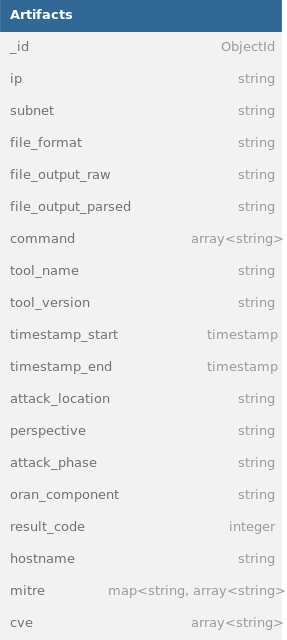
\includegraphics[width=0.5\textwidth]{db-schema}
    \caption{Struktur eines Artefakts in der Datenbank und in Go.}
\end{figure}



